% symmReduc.tex                 Predrag 2010.06.29
% Dresden conference talk
% $Author$ $Date$

\documentclass{beamer}
%\documentclass{powerdot}
%\documentclass{slides}[14pt]
%\pagestyle{empty}
%\normalsize
\usepackage{amsmath}
\usepackage{amssymb}
\usepackage{amscd}
% \usepackage{moreverb}
\usepackage{graphicx}
% \usepackage[all]{xy}
% \usepackage{beamerthemesplit}
\usepackage{moreverb}
\usepackage[all]{xy}

\input macros			   %% loan from John Gibson's snowbird 07 talk
% \input ../../inputs/defsThesis     %% all Vaggelis edits: \renewcommand, etc

% Setup appearance:

\usetheme{Darmstadt}
\usefonttheme[onlylarge]{structurebold}
\setbeamerfont*{frametitle}{size=\normalsize,series=\bfseries}
\setbeamertemplate{navigation symbols}{}


% Standard packages

\usepackage[english]{babel}
\usepackage[latin1]{inputenc}
\usepackage{times}
\usepackage[T1]{fontenc}


% % Setup TikZ
%
% \usepackage{tikz}
% \usetikzlibrary{arrows}
% \tikzstyle{block}=[draw opacity=0.7,line width=1.4cm]

\title{Continuous symmetry reduction for high-dimensional flows}
\author{Evangelos Siminos}
\author[Siminos, Cvitanovi\'c, Davidchack]
{
  \textcolor{green!50!black}{
  {Predrag~Cvitanovi\'c}\inst{1}
  and
  {Evangelos~Siminos}\inst{1,2}
  }
}
\institute
{
  \inst{1}%
  Georgia Institute of Technology
  \and
  \vskip-2mm
  \inst{2}
  CEA/DAM/DIF, Paris
}
\date{30 Jun 2010}

\begin{document}

\begin{frame}
  \titlepage
\end{frame}

\begin{frame}{Die Vorlesung}
{\Large Das Problem}
dynamical description of turbulence?

\bigskip

progress 1990-2010:
\begin{itemize}
 \item flames
 \item hearts
 \item pipes
 \item planes
 \item cosmos
 \item gluons
\end{itemize}
\end{frame}

%\begin{frame}{Outline}
%  \tableofcontents
%\end{frame}


\section[Navier-Stokes]{Navier-Stokes}

\subsection[modern times]{fluid measurements}

\begin{frame}{amazing data! amazing numerics!}
\begin{block}{3D turbulent pipe flow}
\begin{center}
  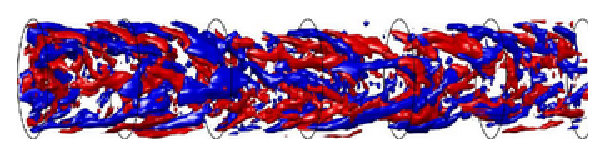
\includegraphics[width=1.0\textwidth,clip=true]
                    {../../figs/vDoorne4}
\end{center}
\end{block}
\end{frame}

\subsection[KSe]{baby Navier-Stokes}
\begin{frame}{flames: \KSe}

\begin{block}{1-dimensional ``Navier-Stokes''}
\[
  u_t + u \triangledown u \,=\, -\triangledown^2 u- \triangledown^4 u
    \,,\qquad   x \in [-L/2,L/2]
    \,,
\]
\end{block}

\bigskip
	\begin{columns}[t]
	\column{.62\textwidth}
describes extended systems such as
\begin{itemize}
 \item reaction-diffusion systems
 \item flame fronts in combustion
 \item drift waves in plasmas, \ldots
\end{itemize}
	\column{.38\textwidth}
\begin{center}
  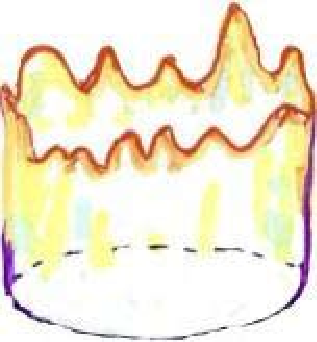
\includegraphics[width=0.70\textwidth,clip=true]
                    {../../figs/flameFlut-fig}
\end{center}
	\end{columns}
\end{frame}

\begin{frame}{a turbulent flame}
\begin{center}
  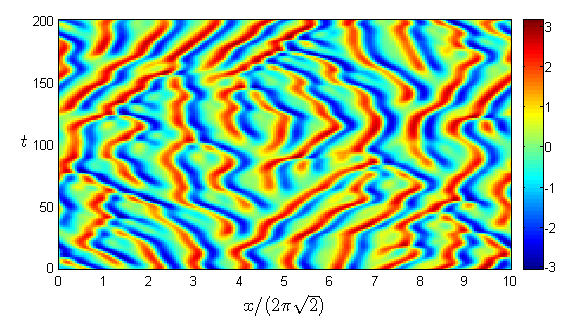
\includegraphics[width=1.00\textwidth,clip=true]
                    {../../figs/ks_largeL_cbar_200}
\end{center}
\end{frame}

\begin{frame}{a peak at a pipe flow experiment}
	\begin{columns}[t]
	\column{.38\textwidth}
    \begin{exampleblock}{a modern pipe flow experiment}
\begin{center}
  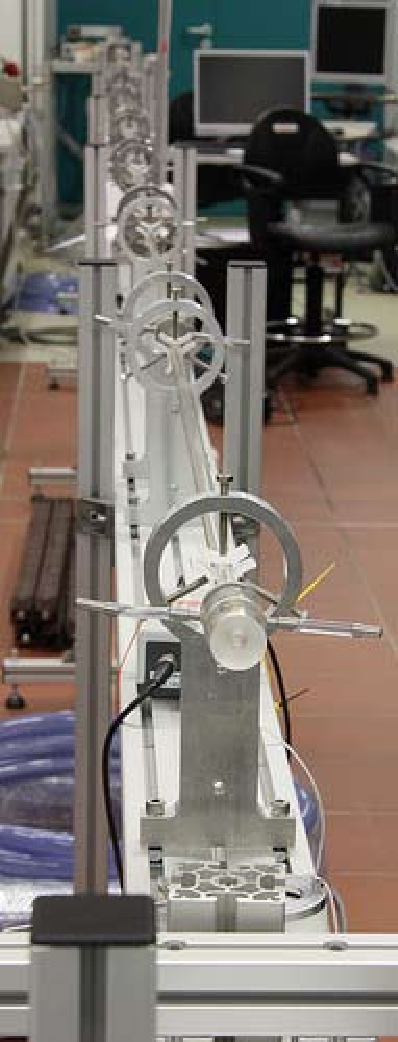
\includegraphics[width=0.45\textwidth,clip=true]
                    {../../figs/pipe}
\end{center}
	\end{exampleblock}
	\column{.6\textwidth}
\begin{center}
  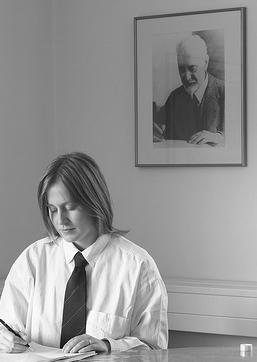
\includegraphics[width=0.60\textwidth,clip=true]
                    {../../figs/Prandtltitos}

{\scriptsize Ludwig Prandtl's office in 2009}
\end{center}
	\end{columns}
{\scriptsize
B. Hof, "Complex Dynamics and Turbulence,"
 \\
one of the groups keeping the Ludwig Prandtl's flame alive in G�ttingen.
}
\end{frame}

\begin{frame}{amazing data! amazing numerics!}
\begin{center}
  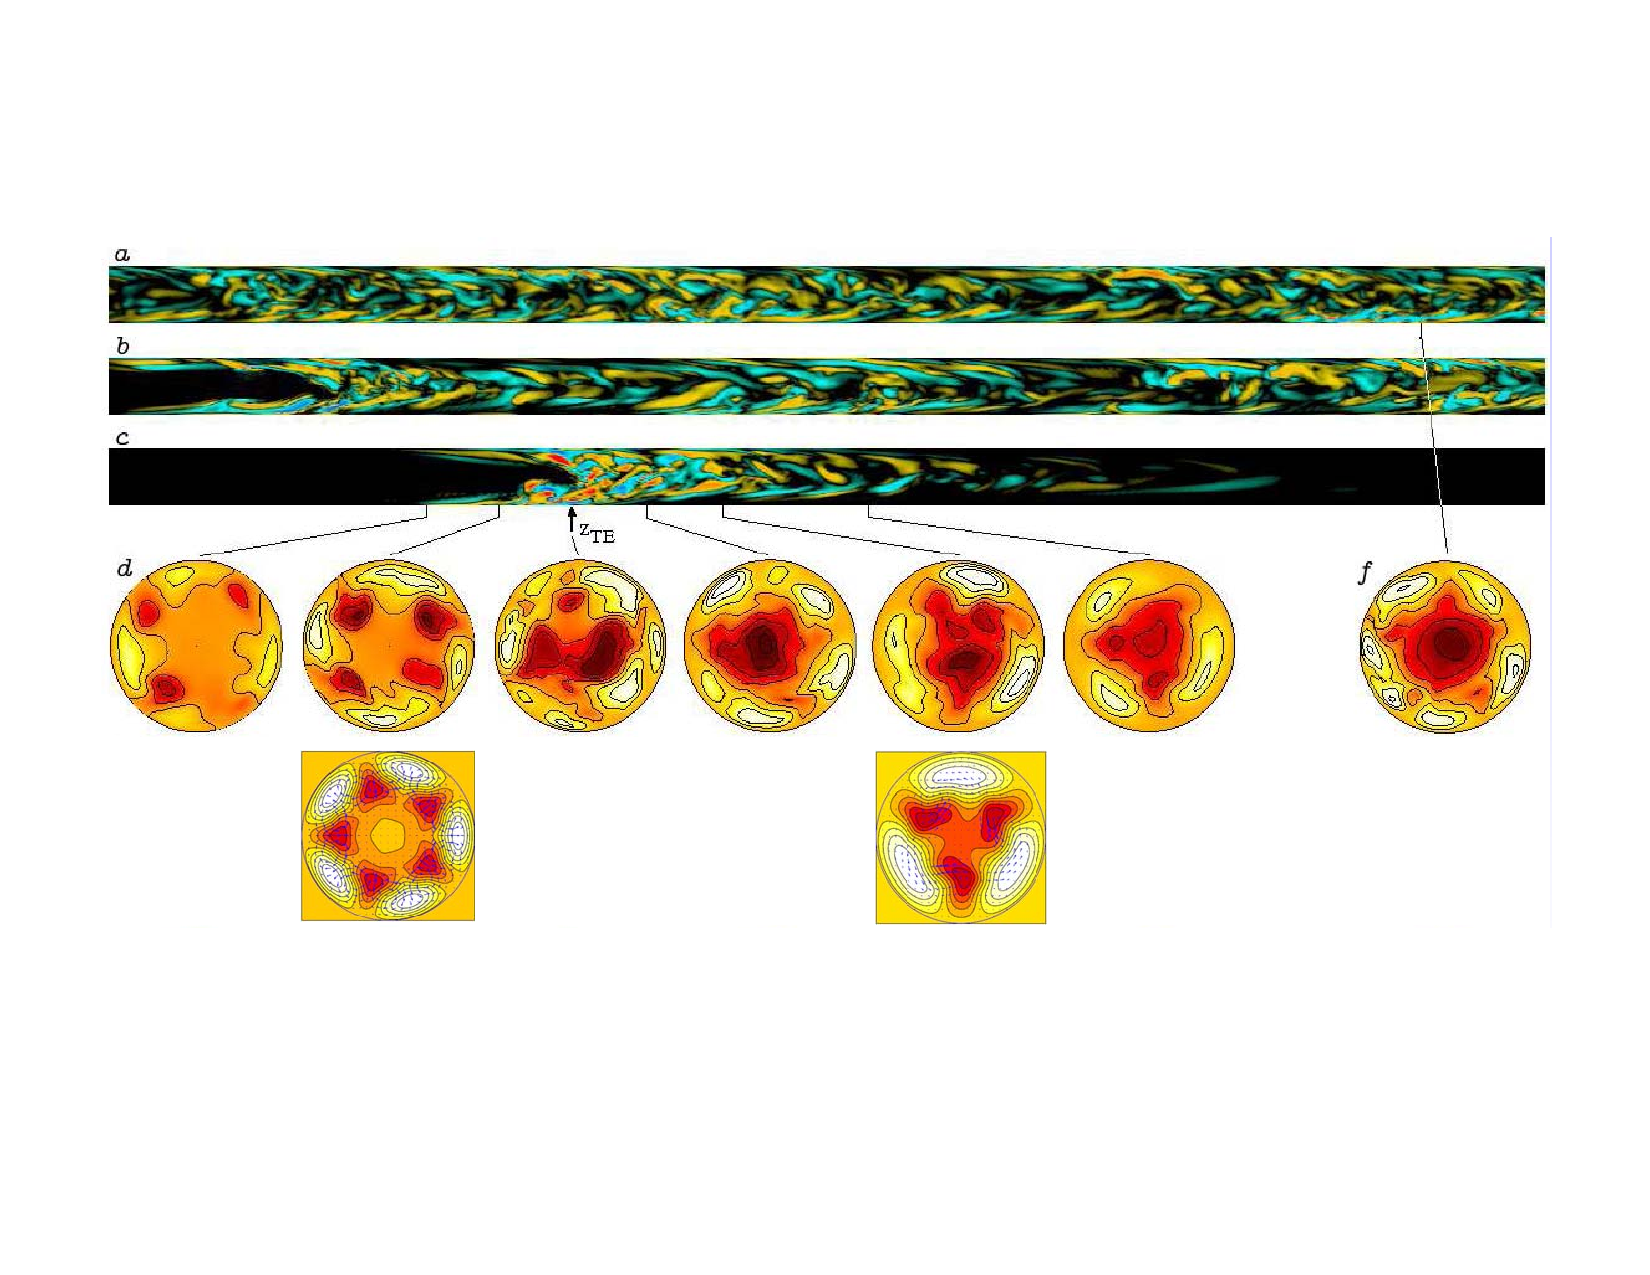
\includegraphics[width=1.0\textwidth,clip=true]
                    {../../figs/pipeSects}
\end{center}

\bigskip

solutions are
\begin{itemize}
 \item rotationally equivariant
 \item translationally equivariant
\end{itemize}

\end{frame}

\begin{frame}{plane Couette flow: G\"ottingen experiment}
\begin{center}
  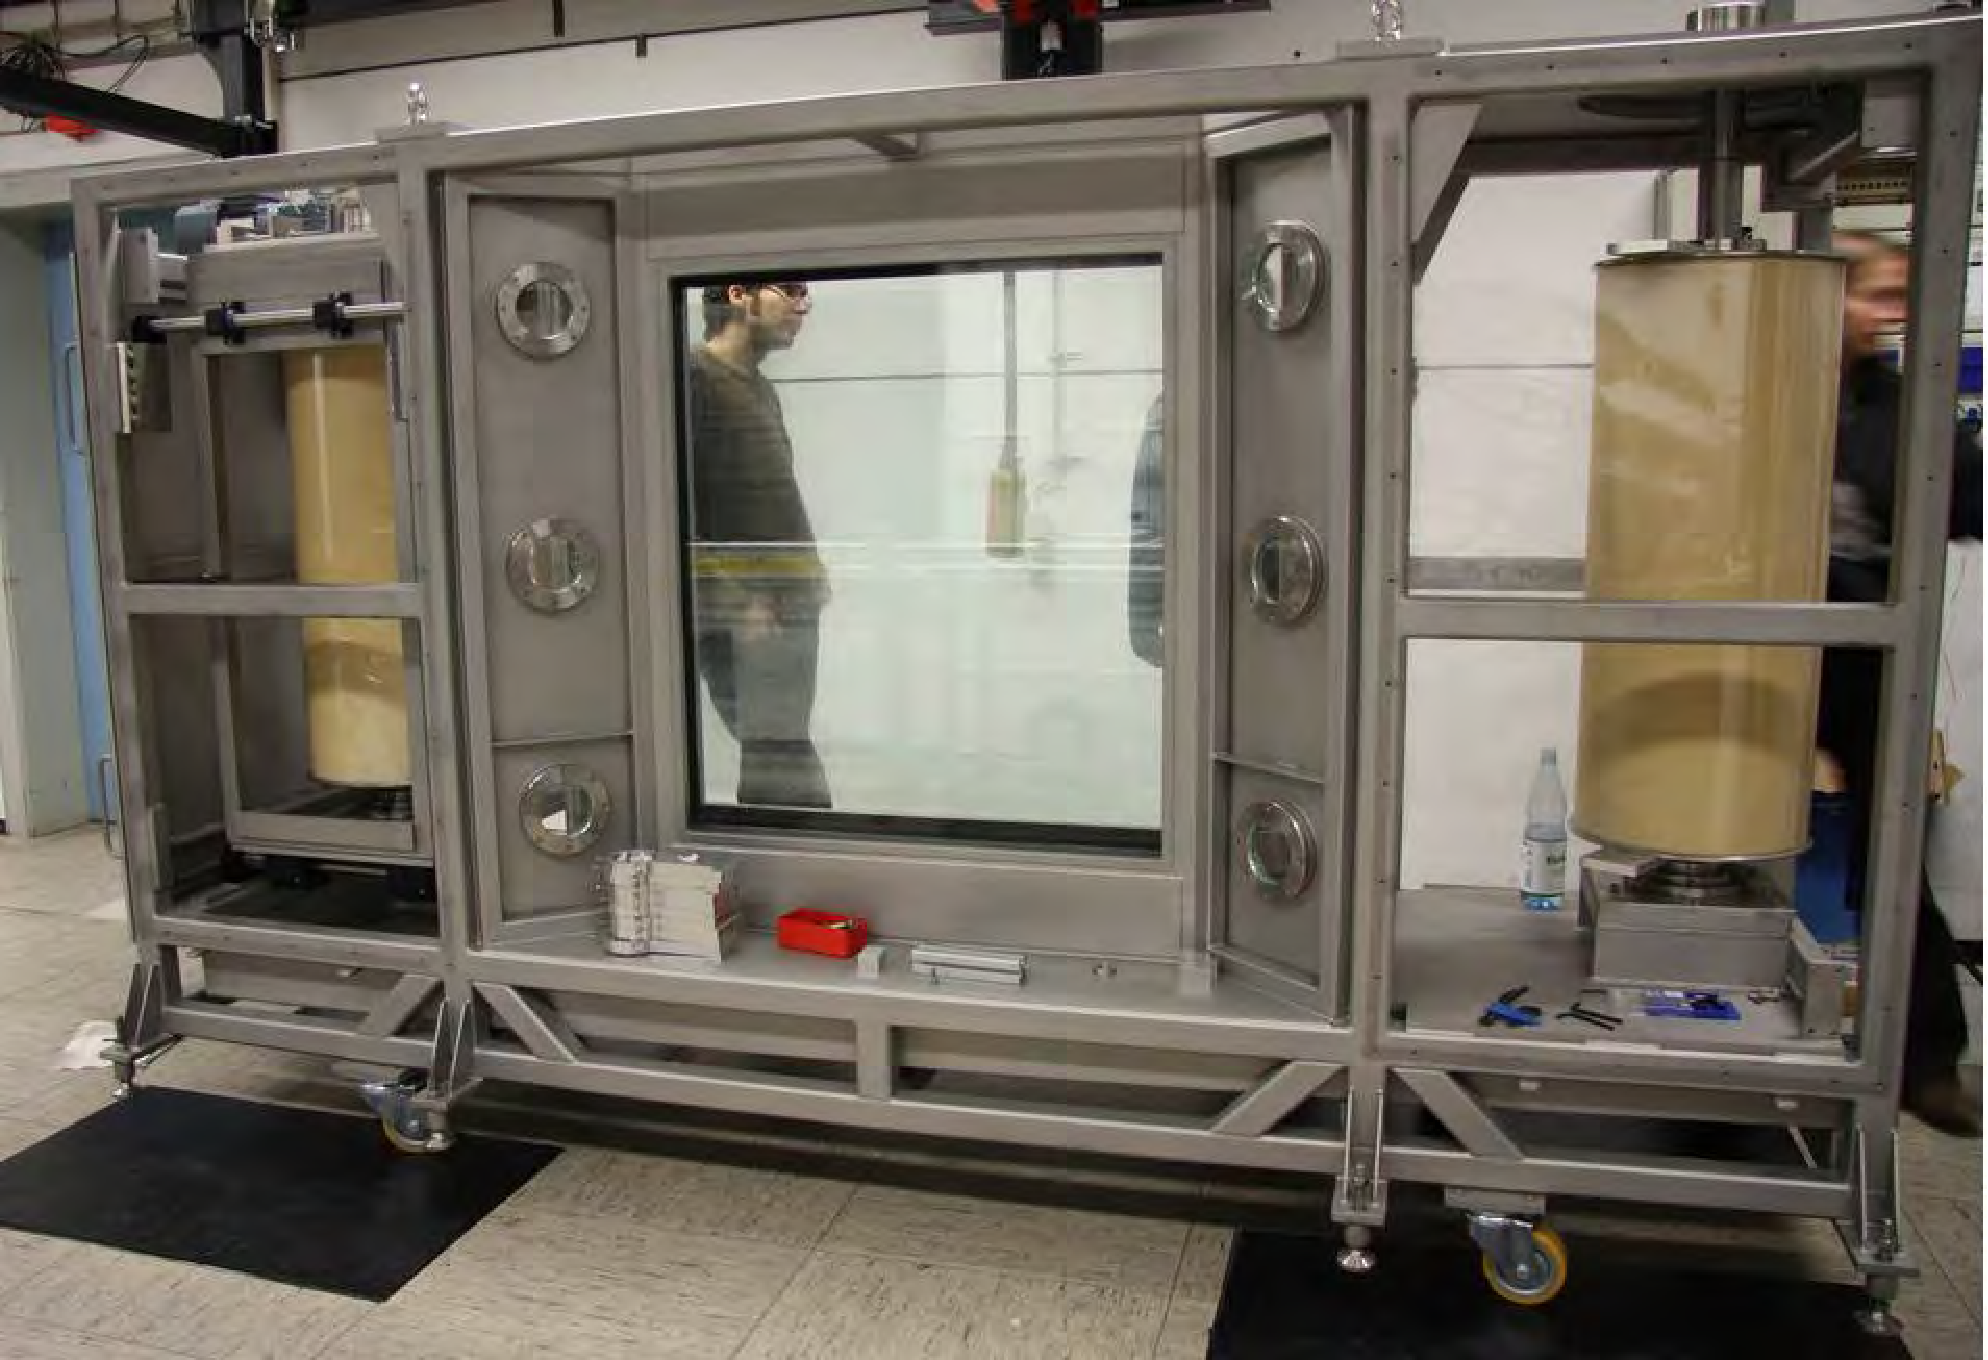
\includegraphics[width=1.00\textwidth,clip=true]
                    {../../figs/planeCouette}
\end{center}
\end{frame}

\begin{frame}{plane Couette flow: fully resolved simulations}
\begin{center}
  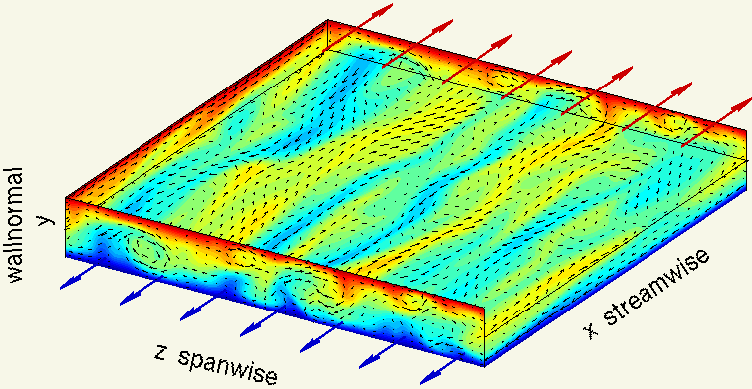
\includegraphics[width=1.00\textwidth,clip=true]
                    {../../figs/ubigbox}
\end{center}
\end{frame}

\subsection{continuous symmetries}

\begin{frame}{symmetries of \KSe}
\only<1->{
with periodic boundary condition
\[
 u(x,t) = u(x+L,t)
\]
         }
the symmetry group is $\On{2}$:
\begin{itemize}
 \item translations: $\Shift_{\shift/L}\, u(x,t)
                     = u(x+\shift,t)\,,\qquad \shift\in\left[-L/2,L/2\right]\,,$
 \item reflections:  $\Refl \, u(x) = -u(-x)\,.$
\end{itemize}

\bigskip

\only<1->{
 translational symmetry $\to$ traveling wave solutions
         }

\bigskip

\only<2->{
traveling (or relative) unstable coherent solutions
are ubiquitous in turbulent hydrodynamic flows
         }

\end{frame}

\begin{frame}{continuous symmetries}
translational symmetry $\Rightarrow$
\begin{itemize}
 \item traveling wave solutions
 \item unstable \rpo s
\end{itemize}
\end{frame}

\begin{frame}{unstable \rpo s}

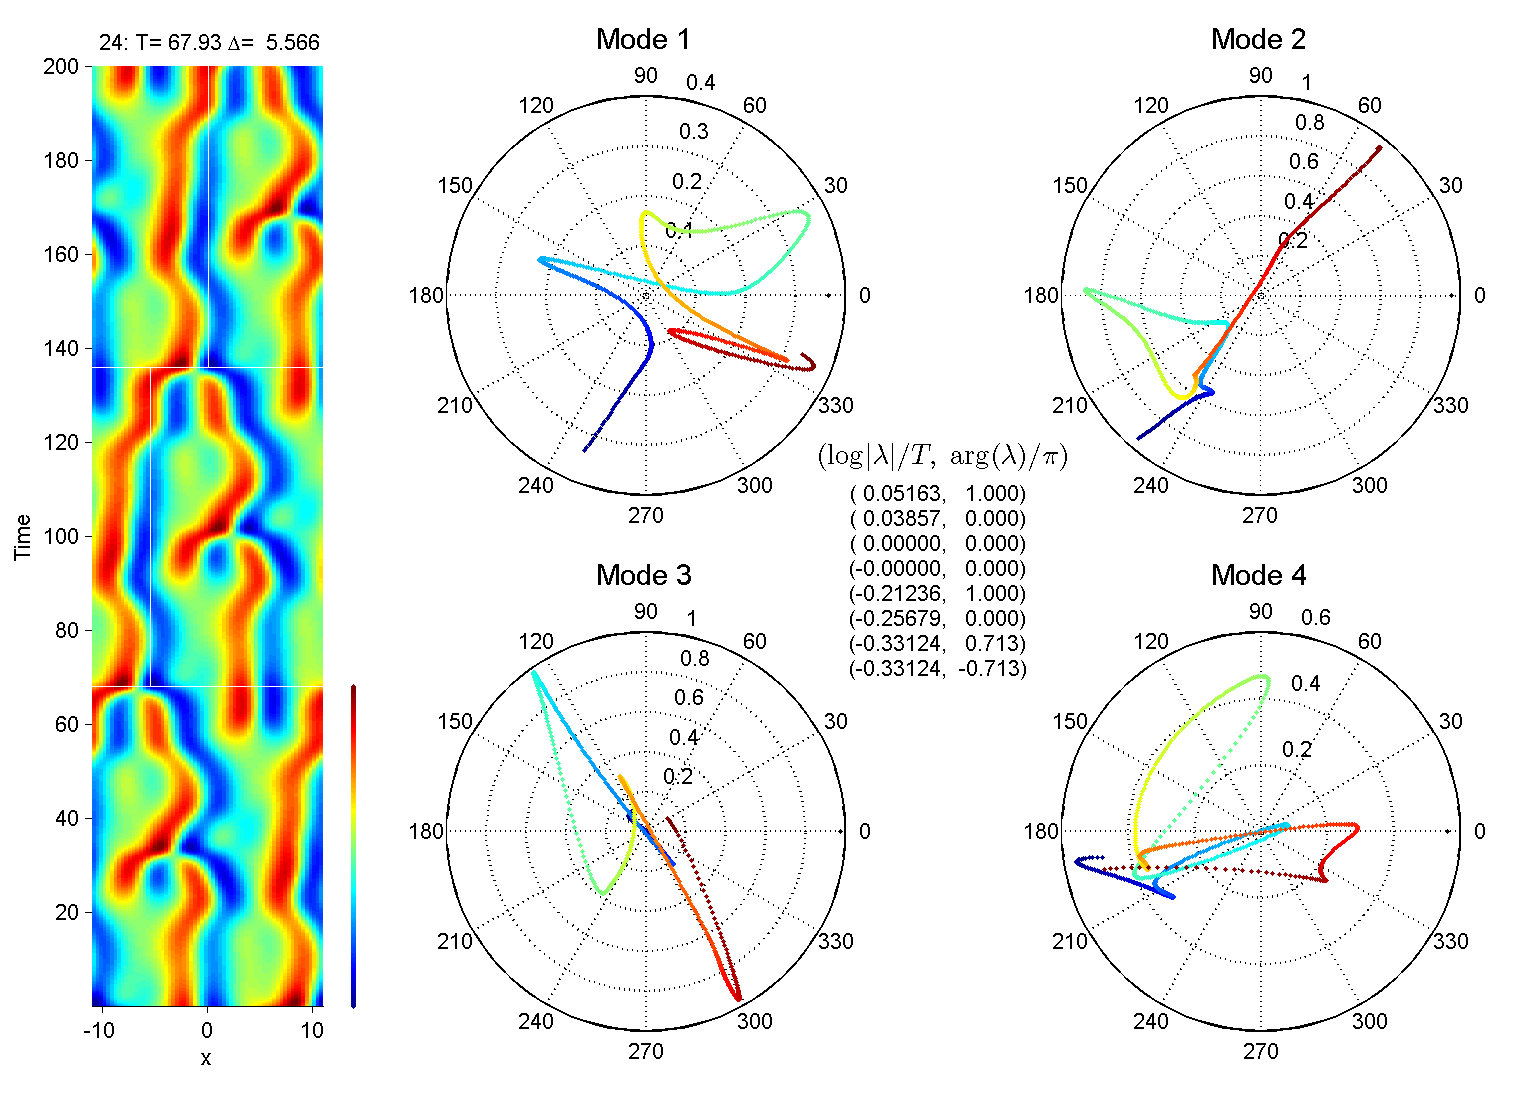
\includegraphics[width=0.75\textwidth]{../../figs/ks22rpo067p93_05p566}

{\scriptsize
\begin{itemize}
 \item have computed 40,000 unstable periodic and \rpo s.
 \item how are they organized?
\end{itemize}
}
\end{frame}

\begin{frame}{continuous symmetries}
\begin{block}{question}
what are the invariant objects that organize phase space in a spatially extended system
with translational symmetry and \textcolor{green}{how do they fit together to form a
skeleton of the dynamics?}
\end{block}
\end{frame}


\section[Dynamicist's view of turbulence]
{Dynamicist's view of  turbulence}

\subsection{PDE's as dynamical systems}

\begin{frame}
\begin{block}{\statesp}
 \begin{itemize}
	\item the space in which all possible states $u$'s live
	\item $\infty$-dimensional:
\\
point $u(x)$ is a function of $x$ on interval $x \in L$.
	\item in practice:
\\
a high but finite dimensional space
     (e.g. through a spectral discretization)
 \end{itemize}
\end{block}
\end{frame}

\begin{frame}{\statesp}
  \begin{block}{take the hint from low dimensional systems}
  \begin{itemize}
  \item low dimensional systems:
  \\
  equilibria, periodic
  orbits organize the long time dynamics.
  \item is this true in extended systems?
  \end{itemize}
 \end{block}
\end{frame}

\subsection{{\cLf} example}

\begin{frame}{from {\cLf} $5D$ attractor $\to$ unimodal map}
	\begin{columns}[t]
	\column{.6\textwidth}
		\only<1>{
			\begin{exampleblock}{{\cLe}}
\scriptsize		
\[
		\left[
					\begin{array}{c}
				\dot{x}_1 \\ \dot{x}_2 \\ \dot{y}_1 \\ \dot{y}_2 \\ \dot{z}
				\end{array}
		\right]
=
		\left[
					\begin{array}{c}
				 -\sigma x_1 + \sigma y_1 \\
				-\sigma x_2 + \sigma y_2 \\
                (\RerCLor-z) x_1 - \ImrCLor x_2 -y_1-e y_2 \\
                \ImrCLor x_1 + (\RerCLor-z) x_2 + e y_1- y_2 \\
				-b z + x_1 y_1 + x_2 y_2
				\end{array}
		\right]
\]
$\RerCLor=28, \ImrCLor=0, b=8/3, \sigma=10, e= 1/10$
			\end{exampleblock}
            \begin{block}{}
  \begin{itemize}
  \item A typical $\{x_1,x_2,z\}$ trajectory
  \item superimposed:
  a trajectory  whose initial
  point is close to the \reqv\ $Q_{1}$
  \end{itemize}
            \end{block}{}
		}
		\only<2>{
			\begin{block}{what to do?}
			\end{block}
			\begin{block}{the goal}
 reduce this messy strange attractor
to a 1-dim\-ens\-ion\-al return map
			\end{block}
			}
		\only<3>{
			\begin{block}{the goal attained}
			\end{block}
			\begin{block}{but it will cost you}
after symmetry reduction; must learn how to
quotient the $\SOn{2}$ symmetry
			\end{block}
			}
	\column{.40\textwidth}
    	\only<1-2>{
		\begin{exampleblock}{attractor}
        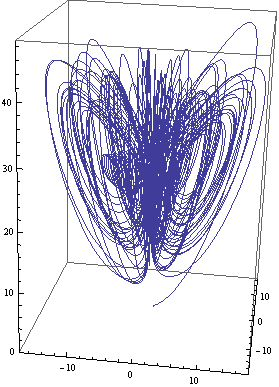
\includegraphics[width=\textwidth,clip=true]
                        {../../figs/CLEx1x2z} %CLEx1x2zRelEqu}
		\end{exampleblock}
        }
        \only<3>{
		\begin{exampleblock}{1D return map!}
        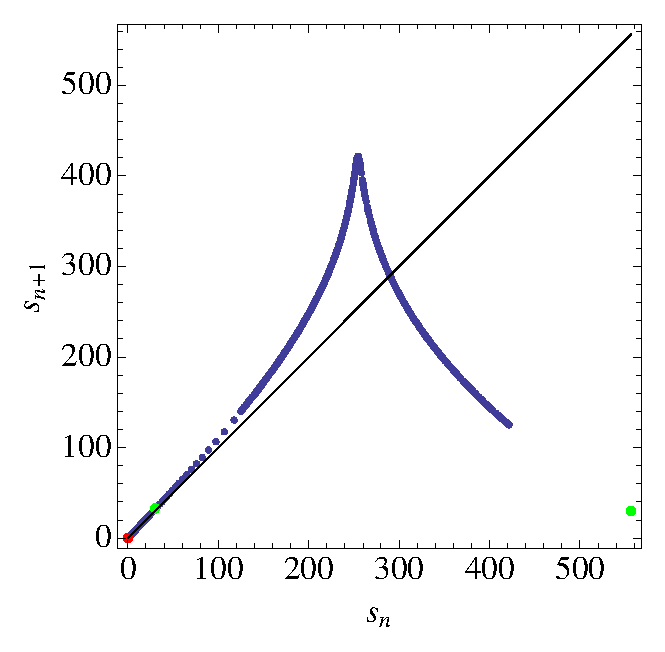
\includegraphics[width=\textwidth,clip=true]
                        {../../figs/CLEipRM}
		\end{exampleblock}
        }
	\end{columns}
\end{frame}

\section[relativity for cyclists]{relativity for cyclists}

\subsection[Lie groups, algebras]{Lie groups, algebras}

\begin{frame}{Lie groups elements, Lie algebra generators}
An element of a compact Lie group:
\[
\LieEl(\gSpace)=e^{\gSpace \cdot \Lg }
	\,,\qquad
\gSpace \cdot \Lg  = \sum \gSpace_a \Lg_a,\; a=1,2, \cdots, N
\] %ee{FiniteRot}
$\gSpace \cdot \Lg$
is a {\em Lie algebra} element,  and $\gSpace_a$ are the parameters
of the transformation.

\end{frame}

\begin{frame}{example: \SOn{2} rotations for \cLe}
\SOn{2} rotation by finite angle \gSpace:
\[
\LieEl(\gSpace) \,=\,  \left(\barr{ccccc}
  \cos \gSpace  & \sin \gSpace  & 0 & 0 & 0 \\
 -\sin \gSpace  & \cos \gSpace  & 0 & 0 & 0 \\
 0 & 0 &  \cos \gSpace & \sin \gSpace   & 0 \\
 0 & 0 & -\sin \gSpace & \cos \gSpace   & 0 \\
 0 & 0 & 0             & 0              & 1
    \earr\right)
\] %{CLfRots}
\end{frame}

\subsection[in/equivariance]{}

\begin{frame}{symmetries of dynamics}
\begin{block}{A flow $\dot{\ssp}= \vel(\ssp)$ is $\Group$-equivariant if}
\[
\vel(\ssp)=\LieEl^{-1} \, \vel(\LieEl \, \ssp)
\,,\qquad \mbox{for all } \LieEl \in {\Group}
\,.
\] %ee{eq:FiniteRot}
\end{block}
\end{frame}

\begin{frame}{foliation by group orbits}
  \begin{columns}
  \column{0.4\textwidth}
\begin{block}{group orbits}
\begin{center}
  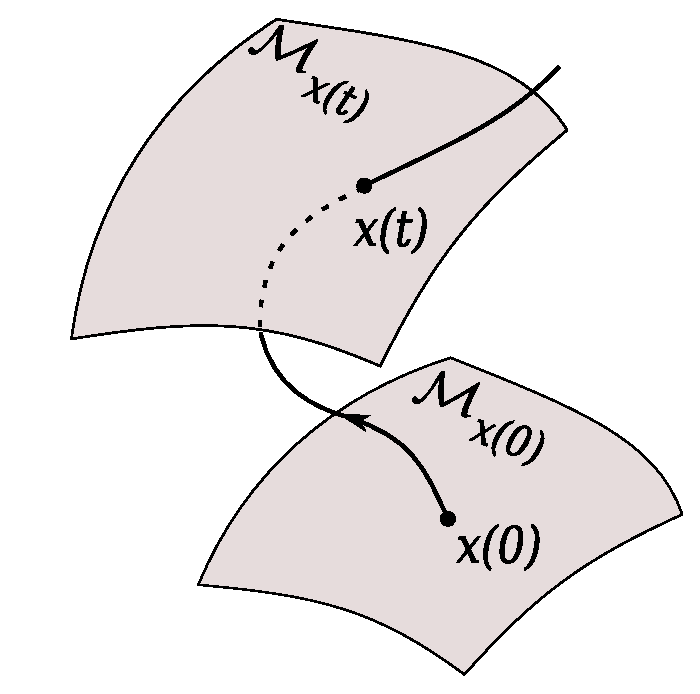
\includegraphics[width=1.00\textwidth,clip=true]
  {../../Fig/BeThTraj}
\end{center}
\end{block}
  \column{0.6\textwidth}
		\only<1>{
\noindent
\emph{group orbit} $\pS_x $ of $\ssp$ is the set of all group
actions
\[
\pS_x = \{\LieEl\,\ssp \mid \LieEl \in {\Group}\}
\]
        }
		\only<2>{
\noindent
group orbit $\pS_{\ssp(0)}$ of \statesp\ point
 $\ssp(0)$, and the group orbit $\pS_{\ssp(t)}$
reached by the trajectory $\ssp(t)$ time $t$ later.
        }
		\only<3>{
\noindent
any point on the manifold $\pS_{\ssp(t)}$ is
equivalent to any other.
        }
		\only<4>{
\noindent
action of a symmetry group
endows the \statesp\ with the structure of a union of group
orbits, each group orbit an equivalence class.
        }
		\only<5>{
\noindent
\textcolor{blue}{the goal}:
\\
replace each group orbit by a unique
point a lower-dimensional {\em \reducedsp}
(or orbit space)
        }
\end{columns}
\end{frame}

\begin{frame}{a traveling wave}
  \begin{columns}
  \column{0.55\textwidth}
%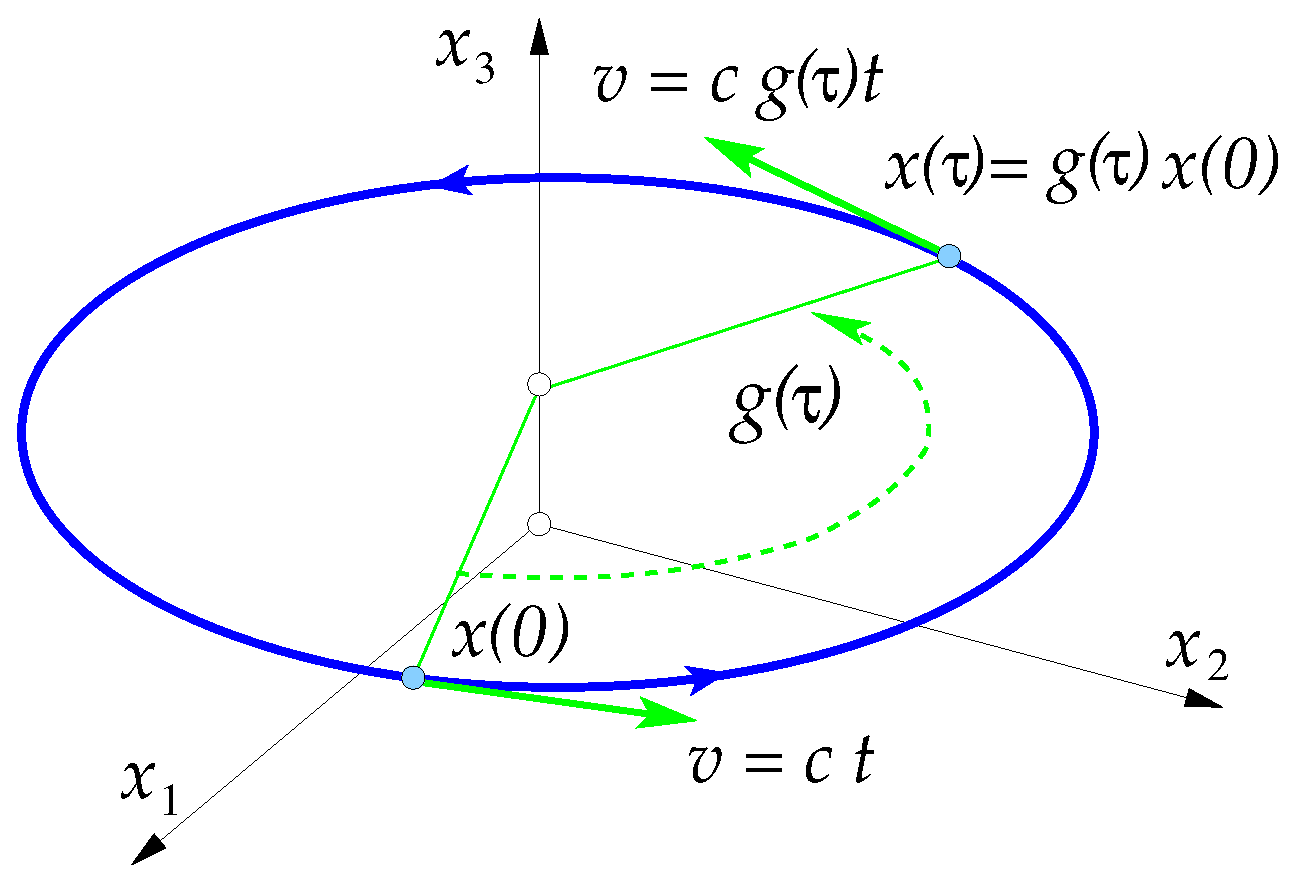
\includegraphics[width=1.0\textwidth,clip=true]
        {../../Fig/reqv}
  \column{0.45\textwidth}
		\only<1,2>{
\noindent
{\em \reqv}
        }
		\only<1>{
\\
 (traveling wave, rotating wave)
\\
$\ssp_{\REQV{}{}}(\tau) \in \pS_{\REQV{}{}}$:
the dynamical flow field points
along the group tangent field, with constant
`angular' velocity  \velRel, and the trajectory stays on the
group orbit
        }
		\only<2>{
\[
\vel(\ssp) \,=\, \velRel \cdot \groupTan(\ssp)
    \,,\qquad
               \ssp \in \pS_{\REQV{}{}}
\]
\bea
\ssp(\tau) &=& \LieEl(-\tau \, \velRel) \, \ssp(0)
    \continue
   &=&
   e^{-\tau \, \velRel \cdot \Lg} \ssp(0)
    \,.
\nnu
\eea %\label{contInvSolns}
        }
		\only<3>{
\noindent
group orbit
$\LieEl(\tau) \, \ssp(0)$ coincides with the dynamical orbit
$\ssp(\tau) \in \pS_{\REQV{}{}}$ and is thus flow invariant
        }
\end{columns}
\end{frame}

\begin{frame}{a \rpo}
  \begin{columns}
  \column{0.55\textwidth}
%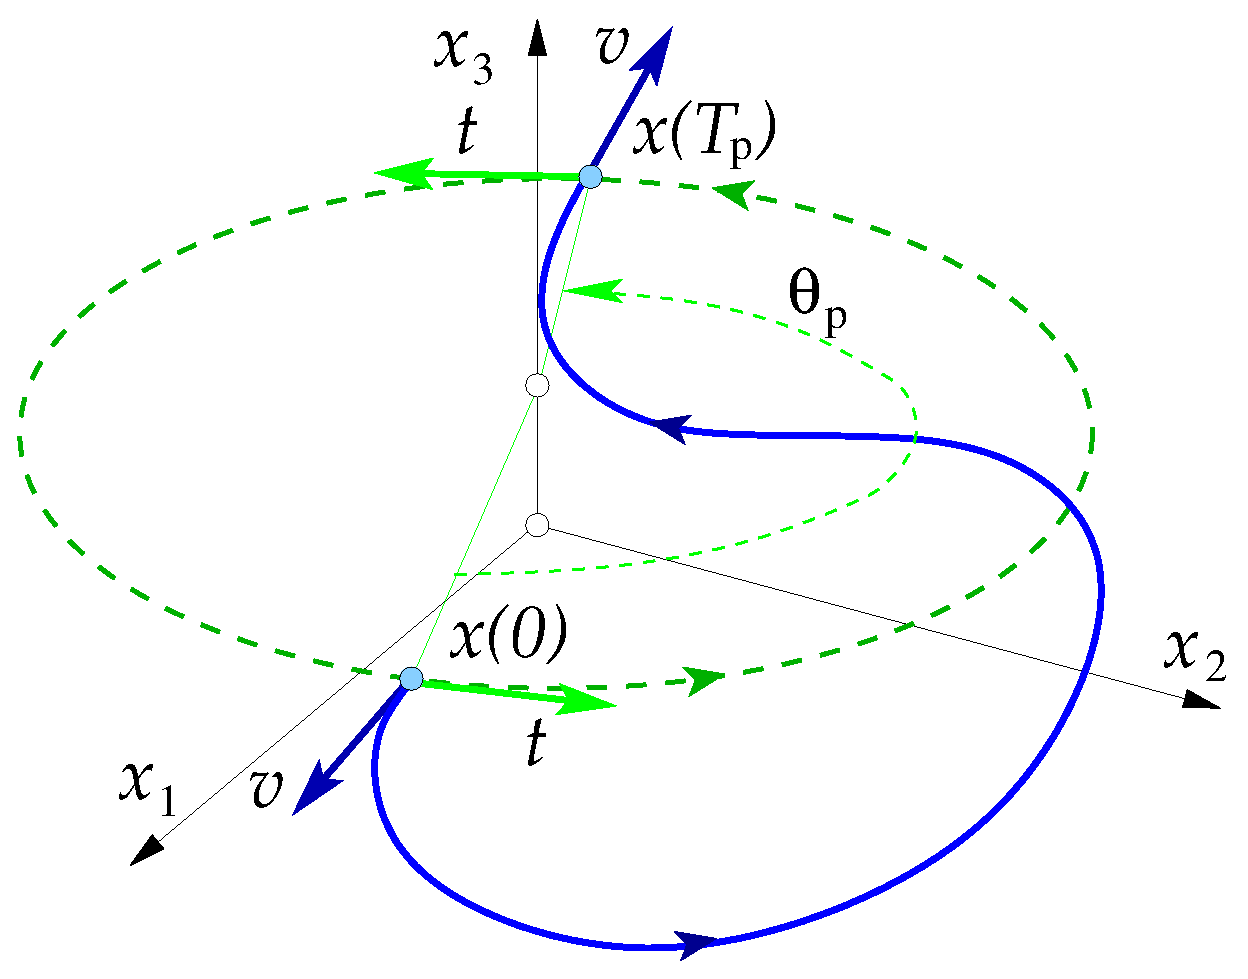
\includegraphics[width=1.0\textwidth,clip=true]
    {../../figs/rpo}
  \column{0.45\textwidth}
		\only<1>{
\noindent
\rpo\
\[
\ssp_p (0) = \LieEl_p \ssp_p (\period{p} )
\] %\label{RPOrelper1}
exactly recurs
at a fixed {\em relative period} $\period{p}$, but
shifted by a fixed group action ${\LieEl_p}$
        }
		\only<2>{
\noindent
{\em \rpo} starts out at $\ssp(0)$ ,
returns to the group orbit of $\ssp(0)$ after
time $\period{p}$, a
rotation of the initial point by $\LieEl_p$
        }
		\only<3>{
\noindent
The group action parameters
\\
$\gSpace = (\gSpace_1,\gSpace_2,\cdots\gSpace_N)$
\\
 are irrational: trajectory sweeps out
ergodically the group orbit without ever closing into a \po.
        }
\end{columns}
\end{frame}

\begin{frame}{relativity for pedestrians}
		\only<1,2>{
\begin{block}{try a co-moving coordinate frame?}
        }
		\only<3>{
\begin{block}{no good global co-moving frame!}
        }
\begin{center}
		\only<1>{
(\textit{a})
  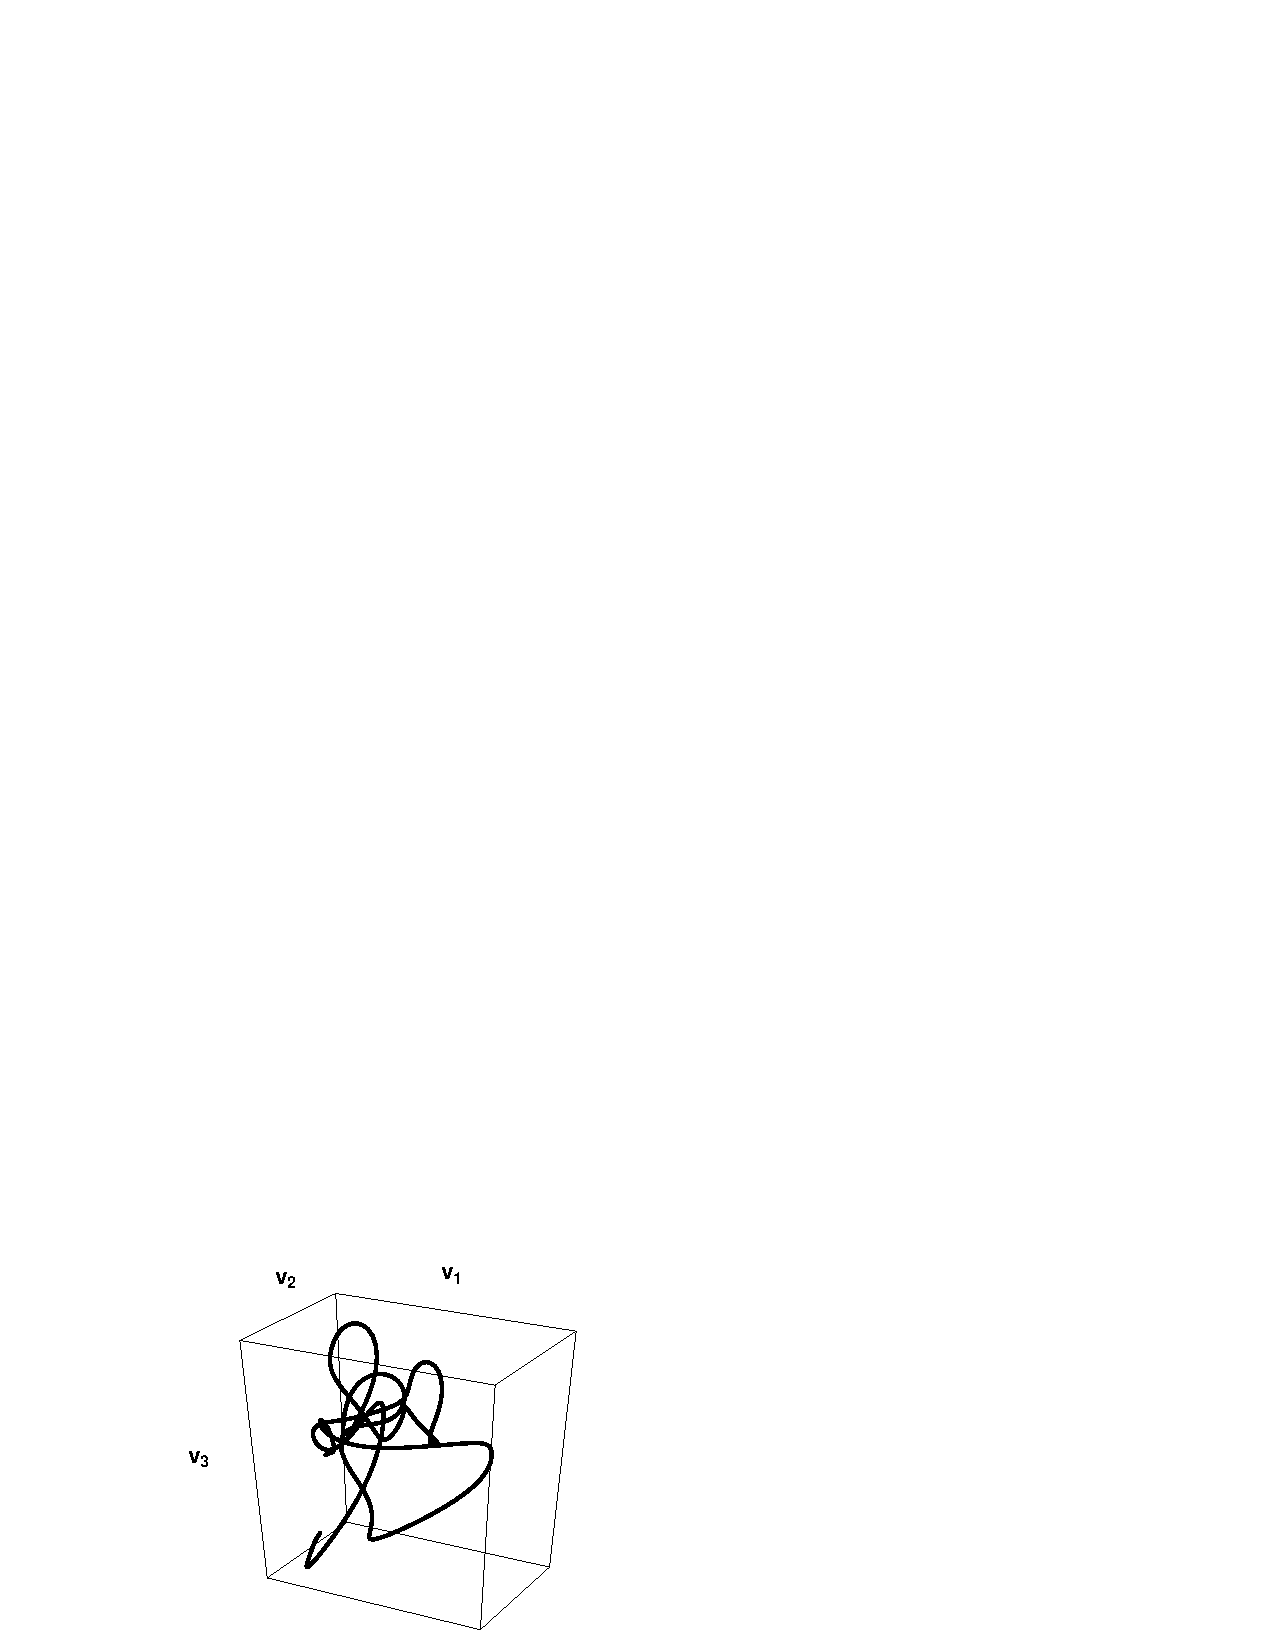
\includegraphics[width=0.40\textwidth,height=0.5\textheight,clip=true]
  {../../figs/ks22rpo033p50_04p045E2}
        }
		\only<2,3>{
(\textit{b})
  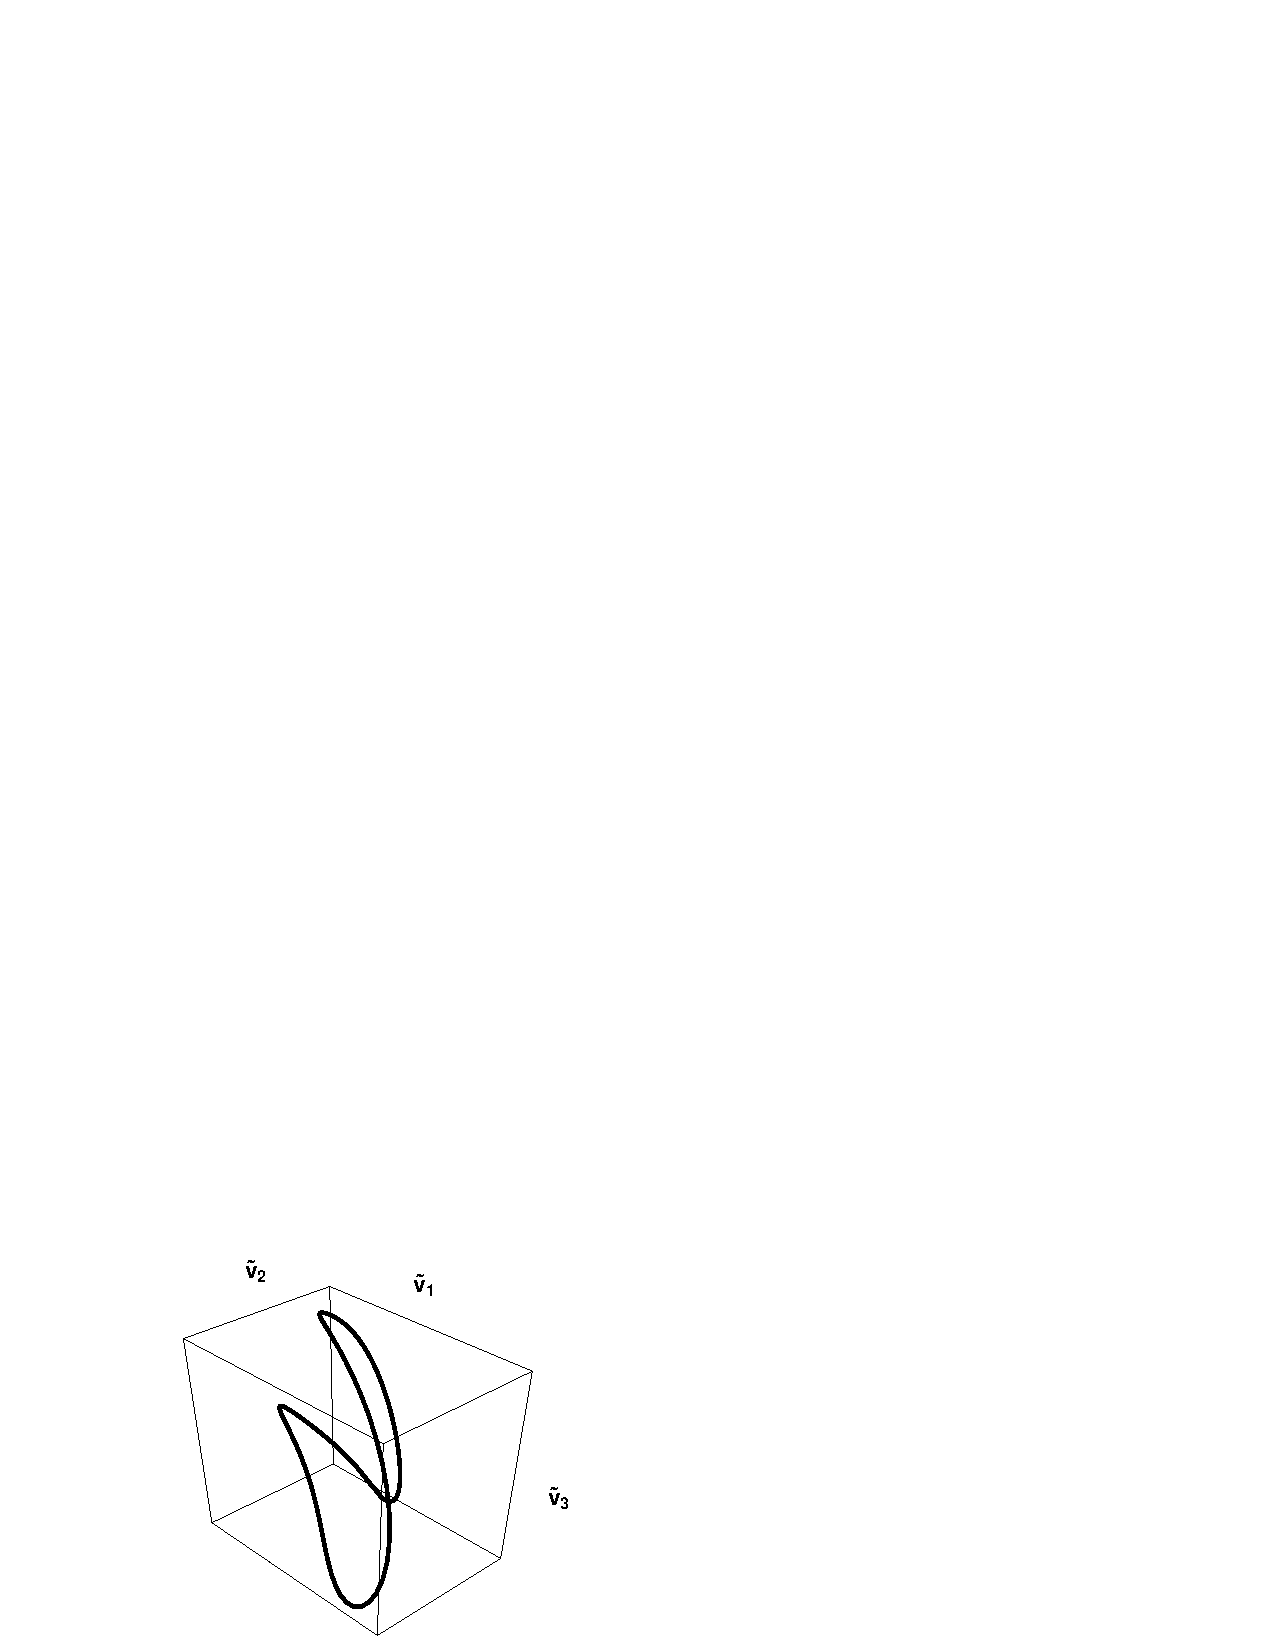
\includegraphics[width=0.40\textwidth,height=0.5\textheight,clip=true]
  {../../figs/ks22rpo033p50_04p045E2CM}
        }
\end{center}
\end{block}
		\only<1,2>{
 A \rpo\ of the Kuramoto-Sivashinsky flow, traced for four periods
 $\period{p}$, projected on
 \\
		\only<1>{
 (a) a stationary \statesp\ coordinate frame
 $\{v_1,v_2,v_3\}$;
        }
		\only<2>{
 (b) a co-moving $\{\tilde{v}_1,\tilde{v}_2,\tilde{v}_3\}$ frame
        }
        }
        \only<3>{
 this is no symmetry reduction at all;
 \\
 all other \rpo s require their own frames,
 \\
 moving at different velocities.
        }
\end{frame}


\section{symmetry reduction}

\begin{frame}{symmetry reduction}
\begin{itemize}
 \item all points related by a symmetry operation are mapped to the same point.
 \item relative equilibria become equilibria and relative periodic orbits become periodic orbits in reduced space.
 \item families of solutions are mapped to a single solution
\end{itemize}
\end{frame}

\begin{frame}{Happy families are all alike;
             \\
             every unhappy family is unhappy in its own way}

\bigskip

everybody, her mother,
\\
and Robert MacKay knows how to do this

\bigskip

except the author of
\end{frame}

\begin{frame}{masters of group theory}
\begin{center}
  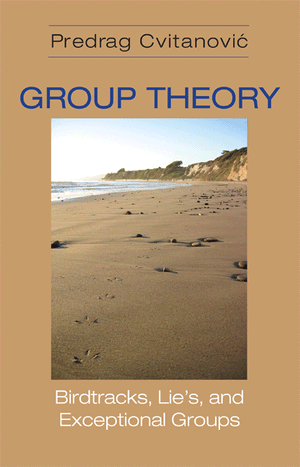
\includegraphics[width=0.40\textwidth,clip=true]
                    {../../figs/coverBtracks}
\end{center}
\end{frame}


\begin{frame}{reduction methods}
\begin{enumerate}
	\item  {\bf Hilbert polynomial basis}: rewrite equi\-vari\-ant
dynamics in in\-vari\-ant coordinates\only<2>{:
\textcolor{green}{global}
        }
	\item {\bf moving frames, or slices}:
cut group orbits by a hypersurface (kind of
Poincar\'e section), each group orbit of
symmetry-equivalent points represented by the single point\only<2>{:
\textcolor{red}{local}
        }
\end{enumerate}
\end{frame}

\subsection{Hilbert polynomial basis}
\begin{frame}{invariant polynomials}
\begin{itemize}
 \item<alert@2-> rewrite the equations in variables invariant
 under the symmetry transformation
 \only<2->{\item or compute solutions in original space and map them to invariant variables}
\end{itemize}
\end{frame}

\begin{frame}{invariant polynomials basis}
        \only<1>{
  \begin{block}{Hilbert basis for \cLe}
\bea
        u_1 &=& x_1^2+x_2^2\,,\qquad\qquad
        u_2 \,=\, y_1^2+y_2^2 \continue
        u_3 &=& x_1 y_2-x_2 y_1\,,\qquad
        u_4 \,=\, x_1 y_1+x_2 y_2 \continue
        u_5 &=& z
\nnu
\eea
  \end{block}
        }
        \only<2>{
  \begin{block}{\cLe\ in invariant polynomial basis}
\bea
\dot{u}_1 &=&2\,\sigma\,(u_3-u_1)\continue
\dot{u}_2 &=&-2\,u_2 -2\,u_3\,(u_5-\rho_1 )\continue
\dot{u}_3 &=&\sigma\,  u_2-(\sigma\,  -1)\,u_3-e\,u_4+u_1\,(\rho_1-u_5)\continue
\dot{u}_4 &=&e\, u_3-(\sigma\, +1)\,u_4\continue
\dot{u}_5 &=&u_3-b\, u_5
\nnu
\eea
  \end{block}
         }
\only<1>{
in\-vari\-ant under $\SOn{2}$ action on a
5-dim\-ens\-ion\-al {\statesp}

\medskip

polynomials related through 1 syzygy:
\[
u_1 u_2 -u_3^2-u_4^2 =0
\] %label{eq:syzLaser}
         }
\only<2>{
A 4-dim\-ens\-ion\-al $\pS/\SOn{2}$ \reducedsp,
a symmetry-in\-vari\-ant representation of the 5-dim\-ens\-ion\-al
\SOn{2} equi\-vari\-ant dynamics
         }
\end{frame}

\begin{frame}{\statesp\ portrait of \cLf}
\begin{block}{drift induced by continuous symmetry}
\begin{center}
  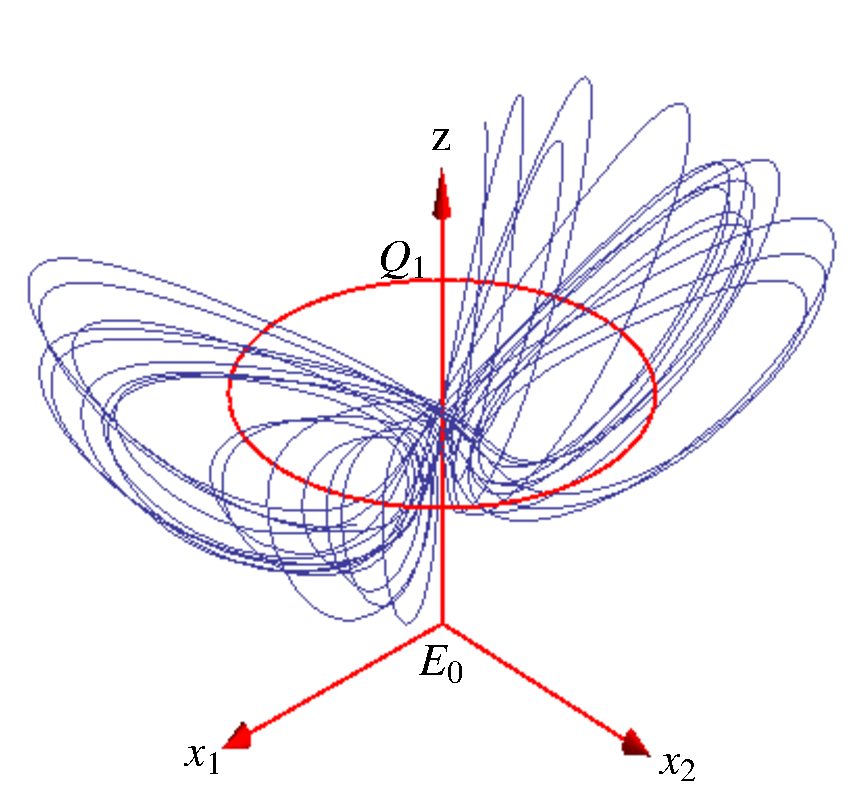
\includegraphics[width=0.45\textwidth,height=0.5\textheight,clip=true]
  {../../figs/CLEchaotic}
  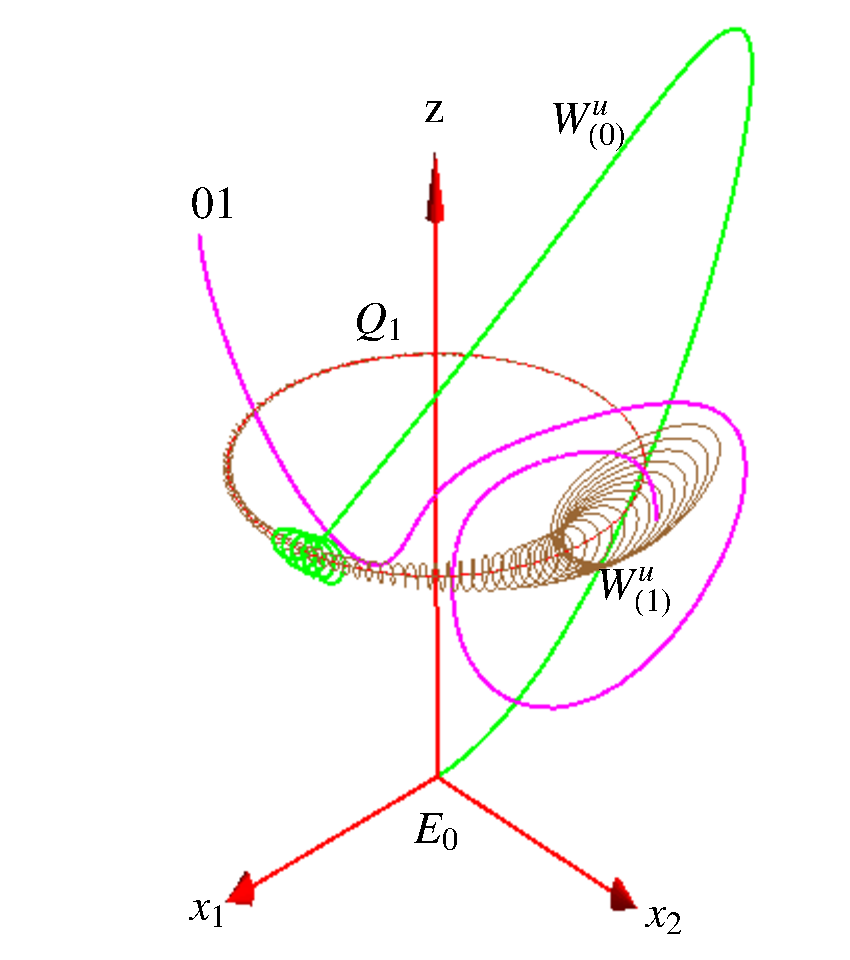
\includegraphics[width=0.45\textwidth,height=0.5\textheight,clip=true]
  {../../figs/CLEcompact}
\end{center}
\end{block}

A generic chaotic trajectory (blue),
the \EQV{0} \eqv,
a representative of its unstable manifold (green),
the $Q_1$ \reqv\ (red), its unstable manifold (brown), and
one repeat of the \cycle{01} \rpo\ (purple).
\end{frame}

\begin{frame}{invariant polynomials basis}
  \begin{block}{\cLe\ in invariant polynomial basis}
\bea
\dot{u}_1 &=&2\,\sigma\,(u_3-u_1)\continue
\dot{u}_2 &=&-2\,u_2 -2\,u_3\,(u_5-\rho_1 )\continue
\dot{u}_3 &=&\sigma\,  u_2-(\sigma\,  -1)\,u_3-e\,u_4+u_1\,(\rho_1-u_5)\continue
\dot{u}_4 &=&e\, u_3-(\sigma\, +1)\,u_4\continue
\dot{u}_5 &=&u_3-b\, u_5
\nnu
\eea
  \end{block}
\only<1>{
the image of the full \statesp\ \reqv\
$Q_{1}$ group orbit is an \eqv\ point,
while the image of a \rpo, such as \cycle{01}, is a
periodic orbit
        }
\end{frame}

\begin{frame}{Hilbert invariant coordinates}
\begin{block}{projected onto in\-vari\-ant polynomials basis}
\begin{center}
(\textit{a})
  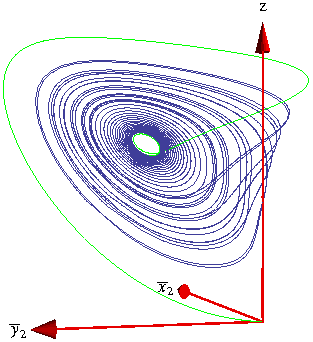
\includegraphics[width=0.40\textwidth,clip=true]
  {../../figs/CLEinvXYZ} %CLEip1}
(\textit{b})
  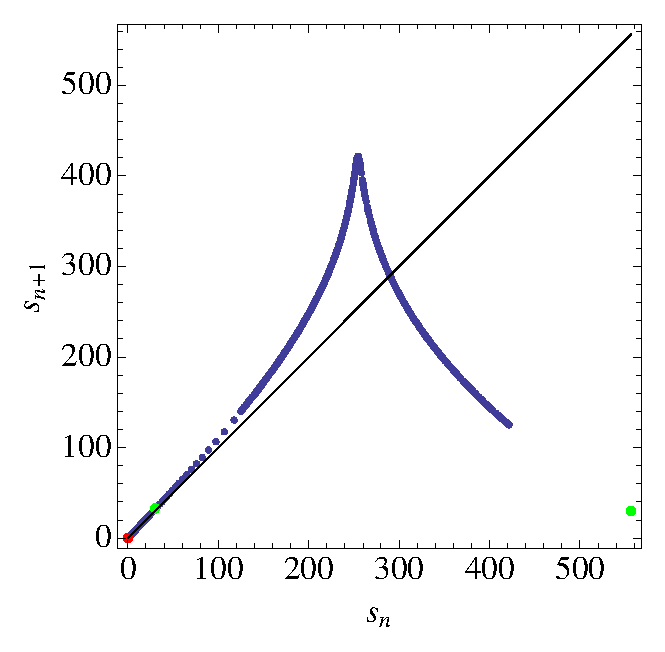
\includegraphics[width=0.45\textwidth,clip=true]
  {../../figs/CLEipRM}
\end{center}
\end{block}
    {\scriptsize
(a) The unstable manifold connection from the \eqv\ $\EQV{0}$ at
the origin to the strange attractor controlled by the
rotation around the \reducedsp\ image of \reqv\ $Q_{1}$;
\\
(b) The return map  projected on in\-vari\-ant polynomials.
    }
\end{frame}

\begin{frame}{higher-dimensional invariant bases? an example}
  \begin{block}
{first 11 invariants for the standard action of $\SOn{2}$}
{\scriptsize
\only<1>{
\[
\begin{array}{l}
  u_1=r_1=\sqrt{b_1^2+c_1^2}  \\
  u_3=\frac{b_2 \left(b_1^2-c_1^2\right)+2 b_1 c_1 c_2}{r_1^2} \\
  u_4=\frac{-2 b_1 b_2 c_1+\left(b_1^2-c_1^2\right) c_2}{r_1^2}\\
  u_5=\frac{b_1 b_3 \left(b_1^2-3 c_1^2\right)-c_1 \left(-3
b_1^2+c_1^2\right) c_3}{r_1^3}  \\
u_6=\frac{-3 b_1^2 b_3 c_1+b_3 c_1^3+b_1^3 c_3-3 b_1 c_1^2 c_3}{r_1^3}
\end{array}
\]
        }
\only<2>{
\[
\begin{array}{ll}
u_7=\frac{b_4
\left(b_1^4-6 b_1^2 c_1^2+c_1^4\right)+4 b_1 c_1 \left(b_1^2-c_1^2\right) c_4}{r_1^4} \\
u_8=\frac{4 b_1
b_4 c_1 \left(-b_1^2+c_1^2\right)+\left(b_1^4-6 b_1^2 c_1^2+c_1^4\right) c_4}{r_1^4}\\
u_9=\frac{b_1
b_5 \left(b_1^4-10 b_1^2 c_1^2+5 c_1^4\right)+c_1 \left(5 b_1^4-10 b_1^2 c_1^2+c_1^4\right) c_5}{r_1^5}\\
u_{10}=\frac{-b_5
c_1 \left(5 b_1^4-10 b_1^2 c_1^2+c_1^4\right)+b_1 \left(b_1^4-10 b_1^2 c_1^2+5 c_1^4\right) c_5}{r_1^5}\\
u_{11}=\frac{b_6
\left(b_1^6-15 b_1^4 c_1^2+15 b_1^2 c_1^4-c_1^6\right)+2 b_1 c_1 \left(3 b_1^4-10 b_1^2 c_1^2+3 c_1^4\right) c_6}{r_1^6}\\
u_{12}=\frac{-2
b_1 b_6 c_1 \left(3 b_1^4-10 b_1^2 c_1^2+3 c_1^4\right)+\left(b_1^6-15 b_1^4 c_1^2+15 b_1^2 c_1^4-c_1^6\right) c_6}{r_1^6}\\
\end{array}
\]
        }
}
  \end{block}

\end{frame}

\begin{frame}{invariant polynomials  - how to find them?}
\begin{itemize}
	\item invariant polynomials (Hilbert basis)\only<2>{:
    computationally prohibitive for high-dimensional flows}
	\only<3->{\item<alert@4-> Cartan moving frame method
    / \mslices\only<5>{:
    singularities}
    }
\end{itemize}
\end{frame}

\subsection{\mslices}

% \begin{frame}{Moving frame method}
%  \begin{block}{Idea}
%   	\begin{itemize}
%  		\item Introduce a \emph{cross-section}: A hypersurface that intersects all group
% 			orbits of a point exactly once.
% 		\item Then given a point $x$ find a map that tells you the transformation parameter(s)
% 			needed to bring $x$ to the cross-section. This is called a moving frame.
% 	\end{itemize}
%  \end{block}
%
%  \begin{block}{For \CLe}
% 	\begin{description}
%  		\item{Cross-section} $x_1=0$, $x_2>0$.
% 		\item{Moving frame} $\theta=\tan^{-1}\frac{x_1}{x_2}$.
% 	\end{description}
%   	
%  \end{block}


% \end{frame}

% \begin{frame}{Moving frame method}
%
% % \[
% % 	\left(\barr{cc} \overline{b}_k \\ \overline{c}_k\earr \right)=\left(\barr{cc}
% % 			    			\cos(k\theta) & -\sin(k\theta)\\
% % 						\sin(k\theta) & \cos(k\theta)\\
% % 			   			\earr\\	
% % 						\right) \left(\barr{cc} b_k \\ c_k\earr\right)\,,\ \ k=1,\ldots N\,.
% % \]
% % with $a_k=b_k+i c_k\,,\ b_k,c_k\in\Rls{}$.
% \end{frame}

\subsection{slice \& dice}

\begin{frame}{Lie algebra generators}
$\Lg_a$ generate infinitesimal
transformations: a set of $N$ linearly independent
$[d\!\times\!d]$ anti-hermitian matrices, $(\Lg_a)^\dagger =
- \Lg_a$, acting linearly on the $d$-dim\-ens\-ion\-al
\statesp\ $\pS$
\begin{block}{example: \SOn{2} rotations for \cLe}
\[
 \Lg \,=\,   \left(\barr{ccccc}
    0  &  1 & 0  &  0 & 0  \\
   -1  &  0 & 0  &  0 & 0 \\
    0  &  0 & 0  &  1 & 0  \\
    0  &  0 &-1  &  0 & 0 \\
    0  &  0 & 0  &  0 & 0
    \earr\right)
\] %ee{CLfLieGen}
\end{block}
The action of \SOn{2}\
on the \cLe\ \statesp\ decomposes into $m=0$ \Group-invariant
subspace ($z$-axis) and  $m=1$ subspace with multiplicity 2.
\end{frame}

\begin{frame}{group tangent fields}
flow field at the \statesp\
point $\ssp$ induced by the action of the group is given by
the set of $N$ \emph{tangent fields}
\[
\groupTan_a(\ssp)_{i}= (\Lg_a){}_{ij} \ssp_j
\] %{GroupTangField}
\end{frame}


\begin{frame}{slice \& dice}
\begin{block}{flow reduced to a slice}
\begin{center}
  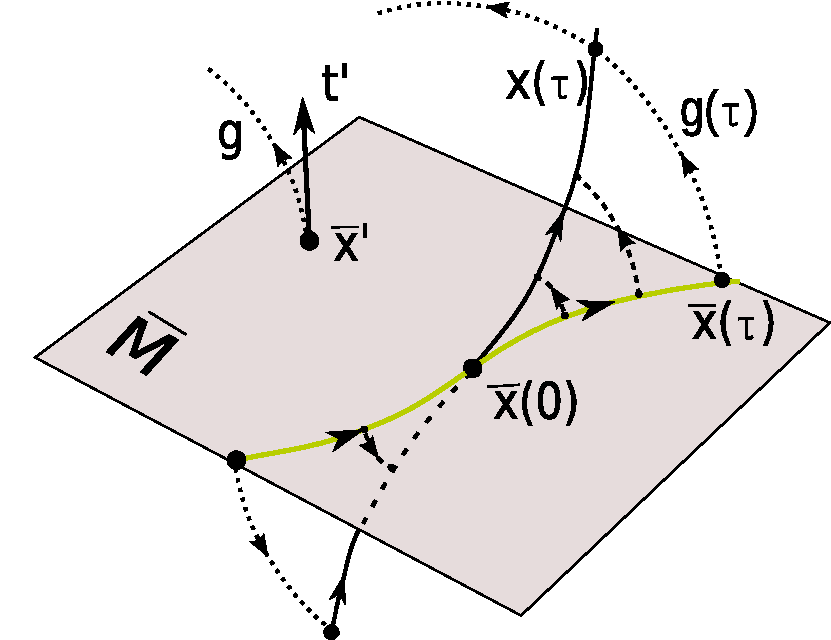
\includegraphics[width=0.45\textwidth,clip=true]
  {../../figs/ReducTraj3}
\end{center}
\end{block}
\Slice\ \pSRed\
through the slice-fixing point $\slicep$,
normal to the group tangent $\sliceTan{}$ at $\slicep$,
intersects
group orbits (dotted lines).
The full
\statesp\ trajectory $\ssp(\tau)$ and the \reducedsp\
trajectory $\sspRed(\tau)$ are equivalent up to a group rotation
$\LieEl(\tau)$.
\end{frame}

\begin{frame}{flow within the slice}
\slice\ fixed by \slicep

\bigskip


	\begin{exampleblock}
          {\reducedsp\ $\pSRed$  flow $\velRed(\sspRed)$}
\bea
\velRed(\sspRed) &=& \vel(\sspRed)
                    \,-\, \dot{\gSpace}(\sspRed)  \cdot \groupTan(\sspRed)
    \,,\qquad\quad \sspRed \in \pSRed
\continue
\dot{\gSpace}_a(\sspRed) &=& (\vel(\sspRed)^T \sliceTan{a})
                       /(\groupTan(\sspRed)^T \cdot \sliceTan{})
\,.
\nnu %\label{EqMotMFrame}
\eea
	\end{exampleblock}

together with the
reconstruction equation for the group phases flow
$\dot{\gSpace}$

\end{frame}

\begin{frame}{slice trouble 1}
\begin{block}{glitches!}
group tangent of a generic trajectory orthogonal
to the slice tangent at a sequence of instants $\tau_k$
\[
\groupTan(\tau_k)^T \cdot \sliceTan{} = 0
\]
\end{block}
\end{frame}

\begin{frame}{slice trouble 1}
\begin{block}{portrait of \cLf\ in \reducedsp}
\begin{center}
(\textit{a})
  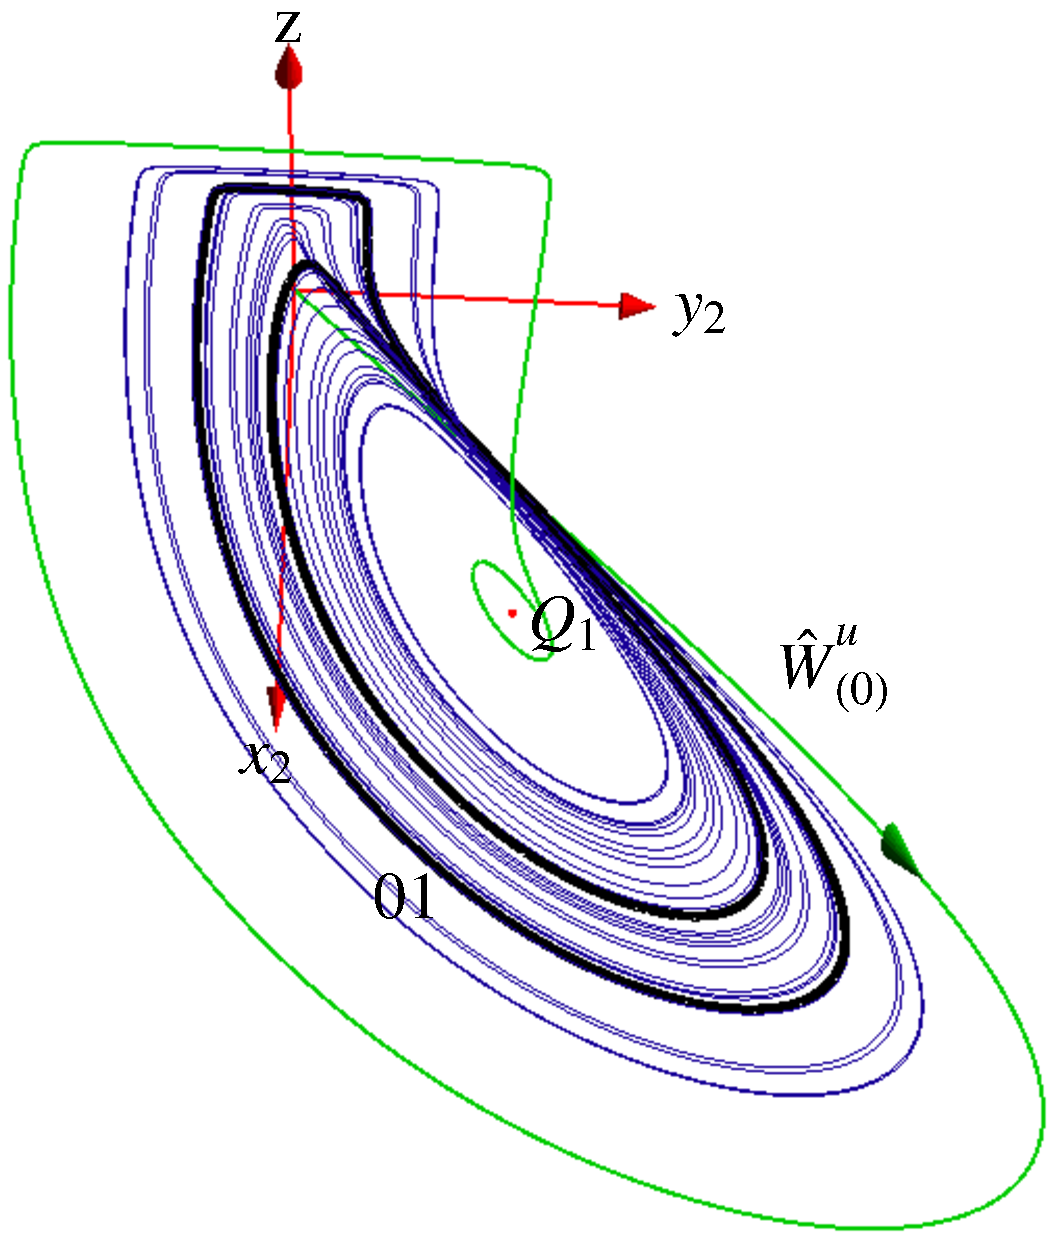
\includegraphics[width=0.40\textwidth,clip=true]
  {../../figs/CLEcoord245}
(\textit{b})
  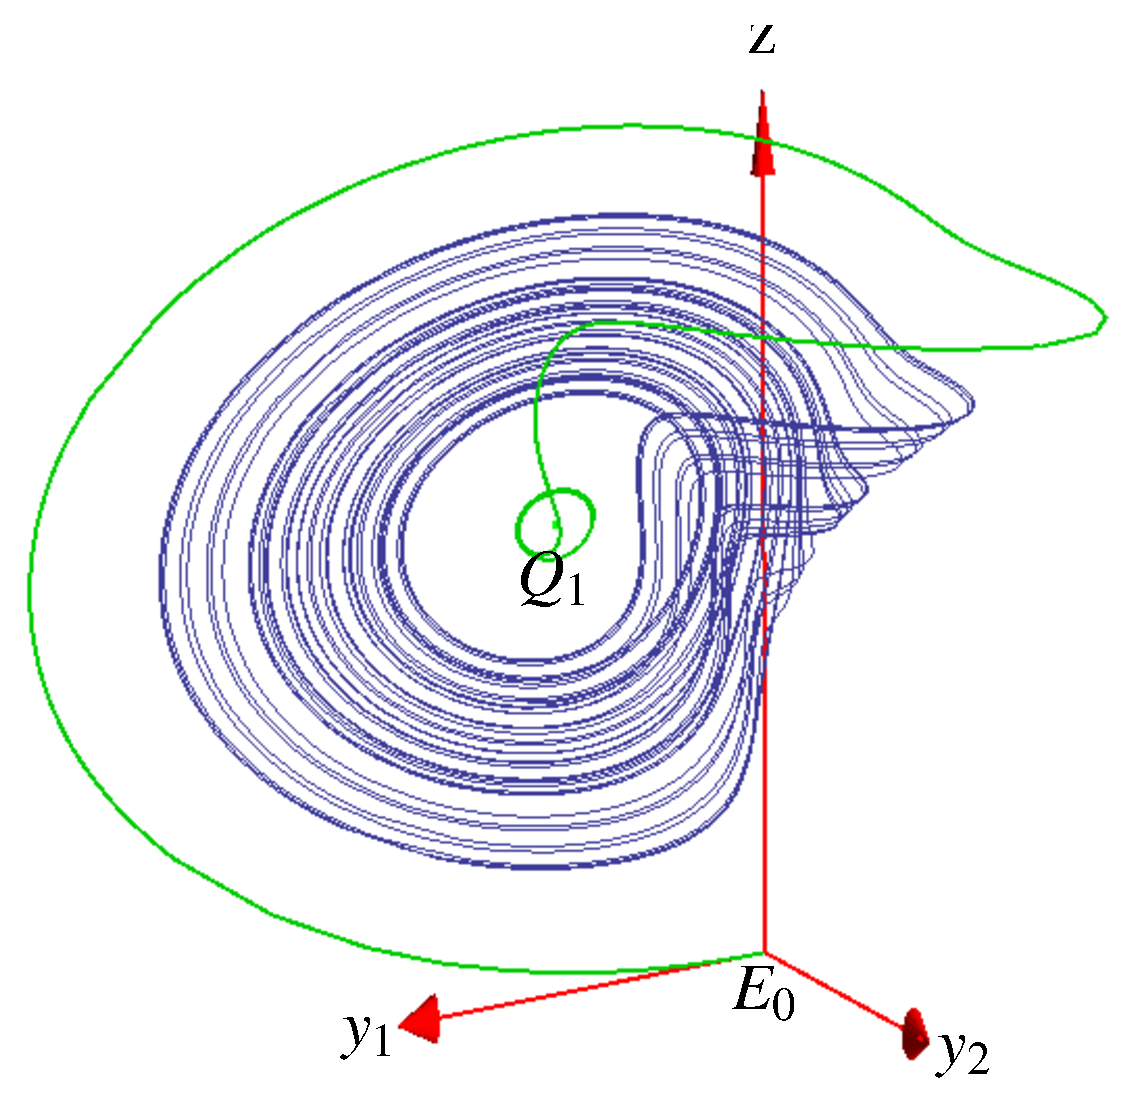
\includegraphics[width=0.45\textwidth,clip=true]
  {../../figs/CLEperpReqb}
\end{center}
\end{block}
all choices of the slice fixing point $\slicep$
exhibit flow discontinuities / jumps
\end{frame}


\begin{frame}{slice trouble 2}
 \begin{columns}
 \column{0.6\textwidth}
\begin{block}{slice cuts a \rpo\ multiple times}
\begin{center}
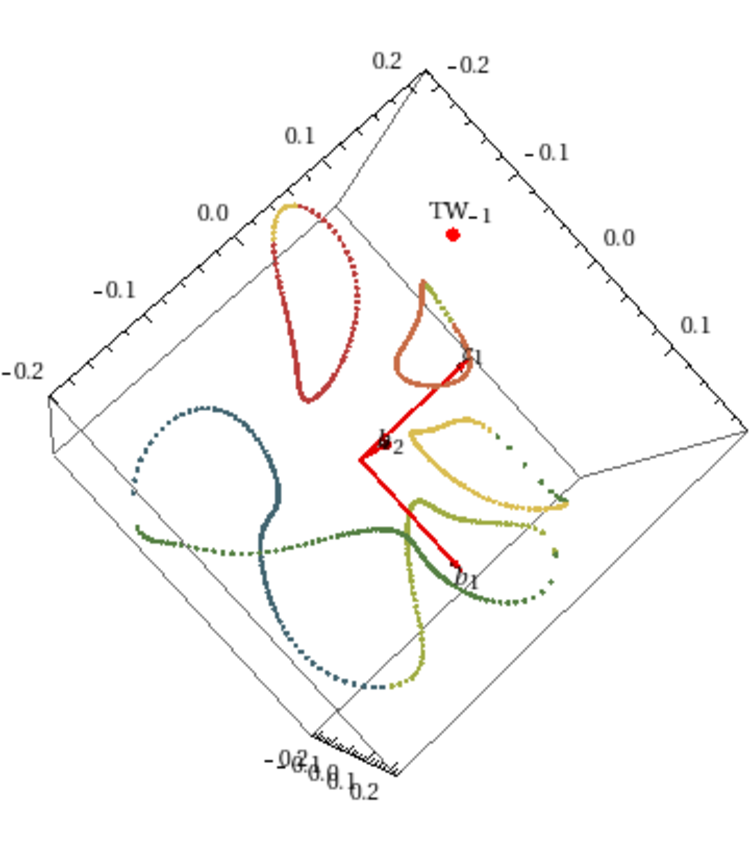
\includegraphics[width=0.80\textwidth]
            {../../figs/ks22rpo16mfAll}
\end{center}
\end{block}
 \column{0.4\textwidth}
\Rpo\ intersects a hyperplane slice in $3$ closed-loop images of
the \rpo\ and $3$ images that appear to connect to a closed
loop.
  \end{columns}
\end{frame}



\section[Summary]{conclusions}

 \begin{frame}{summary}

\begin{block}{conclusion}
  \begin{itemize}
   \item Symmetry reduction by slicing:
   \\
   efficiently implemented, allows
   exploration of high-dimensional flows with continuous
   symmetry.
   \item stretching and folding
  	of unstable manifolds in \reducedsp\ organizes the flow
  \end{itemize}
\end{block}

\begin{block}{to be done}
\begin{itemize}
  \item construct Poincar\'e sections and return maps
  \item find all (relative) periodic orbits up to a given period.
  \item use the information quantitatively (periodic orbit theory).
\end{itemize}
\end{block}

\end{frame}

\begin{frame}{amazing data! amazing numerics! frustration...}
\begin{center}
  
\includegraphics[width=0.60\textwidth,clip=true]
                    {../../figs/ProblemsPill}
\end{center}
\end{frame}


%\begin{frame}{unstable \rpo s}
%\Rpo s (modulated traveling waves) satisfy:
%\[
%  \Shift_{\shift_p/L}u(x,\period{p}) =
%  u(x+\shift_p,\period{p}) = u(x,0) = u_p(x)\,.
%\]
%\Po s satisfy:
%% \[
%%    \Refl u(x+\shift,\period{p}) =
%%   -u(-x-\shift,\period{p}) = u(x+\shift,0) = u_p(x)
%% \]
%\[
%   u(x,\period{p}) = u(x,0)=u_p(x)
%\]
%\end{frame}


\end{document}
